\ifdefined\included
\else
\documentclass[english,a4paper,11pt,twoside]{StyleThese}
\usepackage{amsmath,amssymb}             % AMS Math
\usepackage[T1]{fontenc}
\usepackage[utf8x]{inputenc}
\usepackage{babel}
\usepackage{datetime}

\usepackage{lmodern}
\usepackage{tabularx}
%\usepackage{tabular}
\usepackage{multirow}

\usepackage{subfigure}
\usepackage{fancyvrb}
\usepackage{algorithmic}
\usepackage{algorithm}
\usepackage{mathtools}


\usepackage{hhline}
\usepackage[left=1.5in,right=1.3in,top=1.1in,bottom=1.1in,includefoot,includehead,headheight=13.6pt]{geometry}
\renewcommand{\baselinestretch}{1.05}

% Table of contents for each chapter

\usepackage[nottoc, notlof, notlot]{tocbibind}
\usepackage{minitoc}
\setcounter{minitocdepth}{2}
\mtcindent=15pt
% Use \minitoc where to put a table of contents

\usepackage{aecompl}


% Glossary / list of abbreviations

\usepackage[intoc]{nomencl}
\iftoggle{ThesisInEnglish}{%
\renewcommand{\nomname}{Glossary}
}{ %
\renewcommand{\nomname}{Liste des Abréviations}
}

\newcommand{\accom}[1]{\textcolor{red}{[#1]}}

\makenomenclature

% My pdf code

\usepackage{ifpdf}

\ifpdf
  \usepackage[pdftex]{graphicx}
  \DeclareGraphicsExtensions{.jpg}
  \usepackage[a4paper,pagebackref,hyperindex=true]{hyperref}
  \usepackage{tikz}
  \usetikzlibrary{arrows,shapes,calc}
\else
  \usepackage{graphicx}
  \DeclareGraphicsExtensions{.ps,.eps}
  \usepackage[a4paper,dvipdfm,pagebackref,hyperindex=true]{hyperref}
\fi

\graphicspath{{.}{images/}}

%% nicer backref links. NOTE: The flag ThesisInEnglish is used to define the
% language in the back references. Read more about it in These.tex

\iftoggle{ThesisInEnglish}{%
\renewcommand*{\backref}[1]{}
\renewcommand*{\backrefalt}[4]{%
\ifcase #1 %
(Not cited.)%
\or
(Cited in page~#2.)%
\else
(Cited in pages~#2.)%
\fi}
\renewcommand*{\backrefsep}{, }
\renewcommand*{\backreftwosep}{ and~}
\renewcommand*{\backreflastsep}{ and~}
}{%
\renewcommand*{\backref}[1]{}
\renewcommand*{\backrefalt}[4]{%
\ifcase #1 %
(Non cité.)%
\or
(Cité en page~#2.)%
\else
(Cité en pages~#2.)%
\fi}
\renewcommand*{\backrefsep}{, }
\renewcommand*{\backreftwosep}{ et~}
\renewcommand*{\backreflastsep}{ et~}
}

% Links in pdf
\usepackage{color}
\definecolor{linkcol}{rgb}{0,0,0.4} 
\definecolor{citecol}{rgb}{0.5,0,0} 
\definecolor{linkcol}{rgb}{0,0,0} 
\definecolor{citecol}{rgb}{0,0,0}
% Change this to change the informations included in the pdf file

\hypersetup
{
bookmarksopen=true,
pdftitle="Joint Action for Human-Robot Interaction",
pdfauthor="Sandra DEVIN", %auteur du document
pdfsubject="Thesis", %sujet du document
%pdftoolbar=false, %barre d'outils non visible
pdfmenubar=true, %barre de menu visible
pdfhighlight=/O, %effet d'un clic sur un lien hypertexte
colorlinks=true, %couleurs sur les liens hypertextes
pdfpagemode=None, %aucun mode de page
pdfpagelayout=SinglePage, %ouverture en simple page
pdffitwindow=true, %pages ouvertes entierement dans toute la fenetre
linkcolor=linkcol, %couleur des liens hypertextes internes
citecolor=citecol, %couleur des liens pour les citations
urlcolor=linkcol %couleur des liens pour les url
}

% definitions.
% -------------------

\setcounter{secnumdepth}{3}
\setcounter{tocdepth}{2}

% Some useful commands and shortcut for maths:  partial derivative and stuff

\newcommand{\pd}[2]{\frac{\partial #1}{\partial #2}}
\def\abs{\operatorname{abs}}
\def\argmax{\operatornamewithlimits{arg\,max}}
\def\argmin{\operatornamewithlimits{arg\,min}}
\def\diag{\operatorname{Diag}}
\newcommand{\eqRef}[1]{(\ref{#1})}

\usepackage{rotating}                    % Sideways of figures & tables
%\usepackage{bibunits}
%\usepackage[sectionbib]{chapterbib}          % Cross-reference package (Natural BiB)
%\usepackage{natbib}                  % Put References at the end of each chapter
                                         % Do not put 'sectionbib' option here.
                                         % Sectionbib option in 'natbib' will do.
\usepackage{fancyhdr}                    % Fancy Header and Footer

% \usepackage{txfonts}                     % Public Times New Roman text & math font
  
%%% Fancy Header %%%%%%%%%%%%%%%%%%%%%%%%%%%%%%%%%%%%%%%%%%%%%%%%%%%%%%%%%%%%%%%%%%
% Fancy Header Style Options

\pagestyle{fancy}                       % Sets fancy header and footer
\fancyfoot{}                            % Delete current footer settings

%\renewcommand{\chaptermark}[1]{         % Lower Case Chapter marker style
%  \markboth{\chaptername\ \thechapter.\ #1}}{}} %

%\renewcommand{\sectionmark}[1]{         % Lower case Section marker style
%  \markright{\thesection.\ #1}}         %

\fancyhead[LE,RO]{\bfseries\thepage}    % Page number (boldface) in left on even
% pages and right on odd pages
\fancyhead[RE]{\bfseries\nouppercase{\leftmark}}      % Chapter in the right on even pages
\fancyhead[LO]{\bfseries\nouppercase{\rightmark}}     % Section in the left on odd pages

\let\headruleORIG\headrule
\renewcommand{\headrule}{\color{black} \headruleORIG}
\renewcommand{\headrulewidth}{1.0pt}
\usepackage{colortbl}
\arrayrulecolor{black}

\fancypagestyle{plain}{
  \fancyhead{}
  \fancyfoot{}
  \renewcommand{\headrulewidth}{0pt}
}

%\usepackage{MyAlgorithm}
%\usepackage[noend]{MyAlgorithmic}
\usepackage[ED=MITT - STICIA, Ets=INP]{tlsflyleaf}
%%% Clear Header %%%%%%%%%%%%%%%%%%%%%%%%%%%%%%%%%%%%%%%%%%%%%%%%%%%%%%%%%%%%%%%%%%
% Clear Header Style on the Last Empty Odd pages
\makeatletter

\def\cleardoublepage{\clearpage\if@twoside \ifodd\c@page\else%
  \hbox{}%
  \thispagestyle{empty}%              % Empty header styles
  \newpage%
  \if@twocolumn\hbox{}\newpage\fi\fi\fi}

\makeatother
 
%%%%%%%%%%%%%%%%%%%%%%%%%%%%%%%%%%%%%%%%%%%%%%%%%%%%%%%%%%%%%%%%%%%%%%%%%%%%%%% 
% Prints your review date and 'Draft Version' (From Josullvn, CS, CMU)
\newcommand{\reviewtimetoday}[2]{\special{!userdict begin
    /bop-hook{gsave 20 710 translate 45 rotate 0.8 setgray
      /Times-Roman findfont 12 scalefont setfont 0 0   moveto (#1) show
      0 -12 moveto (#2) show grestore}def end}}
% You can turn on or off this option.
% \reviewtimetoday{\today}{Draft Version}
%%%%%%%%%%%%%%%%%%%%%%%%%%%%%%%%%%%%%%%%%%%%%%%%%%%%%%%%%%%%%%%%%%%%%%%%%%%%%%% 

\newenvironment{maxime}[1]
{
\vspace*{0cm}
\hfill
\begin{minipage}{0.5\textwidth}%
%\rule[0.5ex]{\textwidth}{0.1mm}\\%
\hrulefill $\:$ {\bf #1}\\
%\vspace*{-0.25cm}
\it 
}%
{%

\hrulefill
\vspace*{0.5cm}%
\end{minipage}
}

\let\minitocORIG\minitoc
\renewcommand{\minitoc}{\minitocORIG \vspace{1.5em}}

\usepackage{multirow}
%\usepackage{slashbox}

\newenvironment{bulletList}%
{ \begin{list}%
	{$\bullet$}%
	{\setlength{\labelwidth}{25pt}%
	 \setlength{\leftmargin}{30pt}%
	 \setlength{\itemsep}{\parsep}}}%
{ \end{list} }

\newtheorem{definition}{Définition}
\renewcommand{\epsilon}{\varepsilon}

% centered page environment

\newenvironment{vcenterpage}
{\newpage\vspace*{\fill}\thispagestyle{empty}\renewcommand{\headrulewidth}{0pt}}
{\vspace*{\fill}}

\usepackage{tablefootnote}

\sloppy
\begin{document}
\setcounter{chapter}{1} %% Numéro du chapitre précédent ;)
\dominitoc
\faketableofcontents
\fi

\chapter{Supervision for Human-Robot Interaction}
\minitoc

\label{ch:Sup}

\section{Role of the supervisor in the global architecture}

\label{sec:globalArchi}

One of the goals of my research group at LAAS-CNRS is to build a fully autonomous robot which interacts and performs Joint Actions with humans. To do so, an architecture for human-robot interaction has been developed and is constantly improved by the group. This architecture is composed of several modules and a simplified scheme of it can be found in Fig.~\ref{fig:GlobalArchi}.

\begin{figure}[!h]
	\centering
    \includegraphics[width=0.7\textwidth]{figs/Chapter2/archiGlobal.png}
    \caption{The global architecture for human-robot interaction implemented at LAAS-CNRS.}
    \label{fig:GlobalArchi}
\end{figure}

\paragraph{Sensorimotor layer:}
The lower level of the architecture is composed of modules which allow to communicate and control sensors and actuators. Among others, this layer is composed of modules interpreting sensors data to detect humans and objects and a module allowing to execute given trajectories by calling the adequate actuators.

\paragraph{Situation Assessment:}
The situation assessment is done by a software called TOASTER \cite{milliezThesis}. One of the functionalities of TOASTER is to build and maintain a consistent world state based on data coming from the sensorimotor layer. Geometric computations are done on this world state to compute symbolic predicates concerning the environment (e.g. \textit{<object, isOn, support>}, \textit{<object, isIn, box>}) and agents abilities and behaviors (e.g. \textit{<object, isVisibleBy, human>}, \textit{<object, isReachableBy, robot>}, \textit{human, isLookingToward, object}). TOASTER is also in charge of perspective taking: the previous predicates are constantly estimated and maintained not only from the robot’s point of view but also from the point of view of all humans concerned and perceived in the current context. All the data concerning the world state are stored and accessible through a temporal database.

\paragraph{Geometric Planner:}
In order to perform actions and movements adapted to the human proximity, our architecture is equipped with a geometric task and motion planner called GTP \cite{waldhart2016novel}. GTP allows to compute trajectories as well as objects placements and grasp. It does that at a level that is human understandable and readable by giving access to high level tasks such as Pick or Place while taking into account the human safety and comfort.

\paragraph{Symbolic Planner:}
For the robot to be able to synthesize Shared Plans, our architecture is equipped with HATP (Human-Aware Task Planner), a human-aware HTN (Hierarchical Task Network) task planner which allows the robot to compute and refine a plan both for itself and its humans partners, taking into account a number of social rules \cite{Lallement2014hatp}.
HATP has been specially designed to integrate a number of features that are meant to promote the synthesis of plans that are acceptable by humans and easily if not trivially understandable by them. It allows to specify the humans and robot capabilities in terms of actions they can execute. Several aspects such as human preferences and comfort, estimation of human effort to achieve a task in a given context and "social rules" are used in a cost-based approach to build "sufficiently good" human-robot Shared Plans.

\paragraph{Dialogue Manager:}
In order for the robot to communicate with humans, a basic dialogue manager has been integrated to the architecture. This module allows to give humans information concerning the environment (it verbalize predicates), ask basic questions (as asking if a human want to perform an action) and understand basic answers (mainly yes or no answers, the user can answer with buttons as there is no speech recognition in the system). 


\paragraph{Supervisor:}
The last module of the architecture is the supervisor. It is the one in charge of controlling collaborative activities. It chooses the robot goals and monitors the Shared Plan execution. To do so, it estimates humans mental states concerning the Shared Plan and takes them into account to decide when to perform actions or to communicate (verbally and/or non-verbally). It also interprets the information coming from the Situation Assessment module in order to recognize human actions like Pick or Place with regard to the Shared Plan. This module is an extension of \cite{clodic2009shary} and \cite{fiore2016planning} and is the major technical contribution of this thesis. Its internal architecture will be detailed in the next section.

\section{The supervisor architecture}

\begin{figure}[!h]
	\centering
    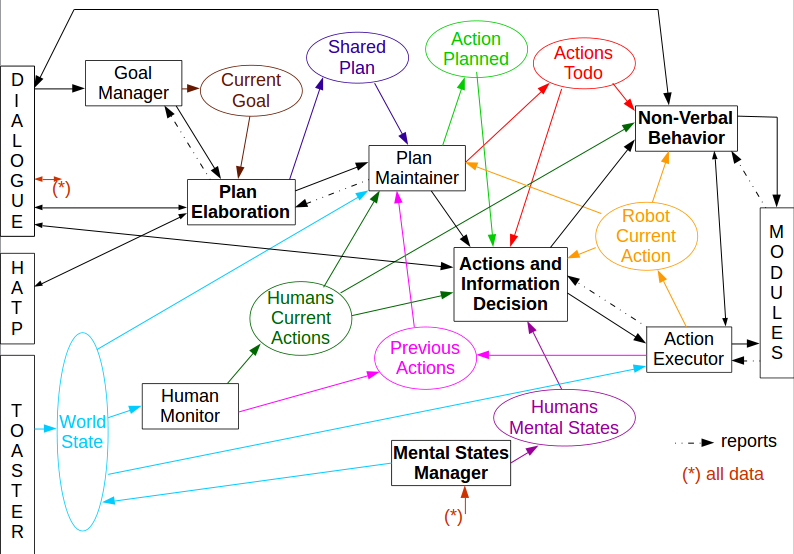
\includegraphics[width=\textwidth]{figs/Chapter2/ArchiSup.png}
    \caption{Architecture of the supervisor.}
    \label{fig:archiSup}
\end{figure}

The supervisor is composed of several modules and is fully implemented in ROS\footnote{http://www.ros.org/}. The complete scheme of its architecture can be found in Fig.~\ref{fig:archiSup}, however, as the figure is quite complex, each composing part of the supervisor will be represented and described individually in the next subsections. 

\subsection{Goal Manager}

The goal manager allows the robot to select and prioritize goals. It maintains a priority list of goals to perform. This list is updated with insert, abort or halt commands from dialogue or command line.

\begin{figure}[!h]
	\centering
    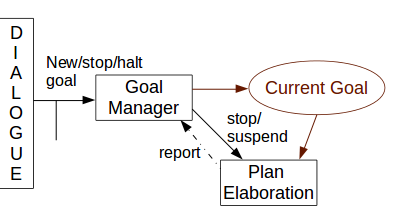
\includegraphics[width=0.5\textwidth]{figs/Chapter2/GoalManager.png}
    \caption{Interaction of the Goal Manager with the rest of the supervisor.}
    \label{fig:goalManager}
\end{figure}

The chosen goal is published in order for the Plan Elaboration module to find a Shared Plan to perform it. The module sends stop and suspend orders to the Plan Elaboration from which it receives reports concerning the success of the plan or the impossibility to find a plan.

This module is, for now, really basic. An interesting extension would be to integrate data coming from an intention recognition module concerning humans activities. This will allow the robot to choose if it should proactively offer its help based on this data and the goal orders it received. 

\subsection{Plan elaboration}

\begin{figure}[!h]
	\centering
    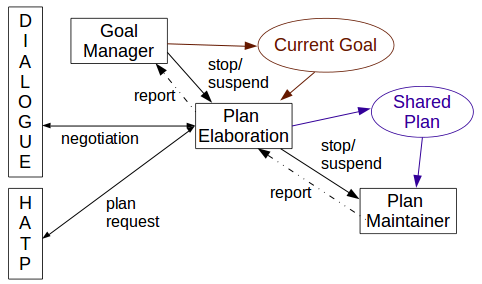
\includegraphics[width=0.6\textwidth]{figs/Chapter2/PlanElaboration.png}
    \caption{Interaction of the Plan Elaboration with the rest of the supervisor.}
    \label{fig:planElaboration}
\end{figure}

Once a goal received from the Goal Manager, the Plan Elaboration module is in charge of finding a Shared Plan to perform it. To do so, the module is able to call HATP (the Human Aware Task Planner described in Sec.~\ref{sec:globalArchi}) to compute a plan and the dialogue module to validate the plan or ask for missing information. One of the contributions of this thesis concerns the elaboration of more flexible Shared Plans where some decisions are left to the execution. This work is in part done in this module and will be developed in Chapter~\ref{ch:SP}.

The computed Shared Plan is then published in order for the Plan Maintainer module to deal with it. The stop and suspend orders received from the Goal Manager are transmitted to the Plan Maintainer module from which it receives reports concerning the success, failure or need of adaptation of the Shared Plan.

\subsection{Plan Maintainer}

The Plan Maintainer module is in charge of monitoring the execution of the Shared Plan based on the current world state and current and past actions. It publishes the list of actions from the Shared Plan which need to be performed at a given moment and the list of actions from the Shared Plan which need to be done later. It also checks the consistency of the plan and reports to the Plan Elaboration module in case of failure or unexpected situations.

\begin{figure}[!h]
	\centering
    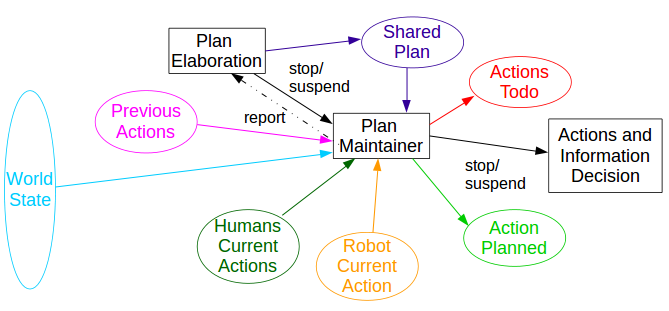
\includegraphics[width=0.8\textwidth]{figs/Chapter2/PlanMaintainer.png}
    \caption{Interaction of the Plan Maintainer with the rest of the supervisor.}
    \label{fig:planMaintainer}
\end{figure}

\subsection{Human Monitor}

The Human Monitor module allows to interpret the current world state which contains humans activity information in order to recognize basic humans actions like Pick or Place. This module is, for now, really basic as it is based mainly on distances between humans and objects. However, there is room for improvements by taking into account the context (e.g. the action the agent is supposed to perform) during action recognition or using probabilistic models.


\begin{figure}[!h]
	\centering
    \includegraphics[width=0.4\textwidth]{figs/Chapter2/HumanMonitor.png}
    \caption{Interaction of the Human Monitor with the rest of the supervisor.}
    \label{fig:humanMonitor}
\end{figure}

\subsection{Mental State Manager}

The Mental State Manager estimates the humans mental states concerning the current goal and Shared Plan. It bases its reasoning on all data published by the other supervisor modules and on the world states from all agents point of view given by TOASTER (see Sec.~\ref{sec:globalArchi}). This work is one of the thesis contribution and will be developed in Chapter \ref{ch:MS}. The composition of the estimated mental states will be given in Sec.~\ref{sec:data}. 

\begin{figure}[!h]
	\centering
    \includegraphics[width=0.5\textwidth]{figs/Chapter2/MSManager.png}
    \caption{Interaction of the Mental State Manager with the rest of the supervisor.}
    \label{fig:MSManager}
\end{figure}

\subsection{Robot Decision}

The Robot Decision module allows the robot to decide which action to execute and which information to give. Its decisions are based on the lists of current, planned and to execute actions as well as on the humans mental states. The way the robot uses these mental states to give pertinent information to humans is one of the thesis contribution and will be developed in Chapter \ref{ch:MS}. The decision of which action to execute has also been studied in this thesis and will be developed in Chapter \ref{ch:SP}.

\begin{figure}[h]
	\centering
    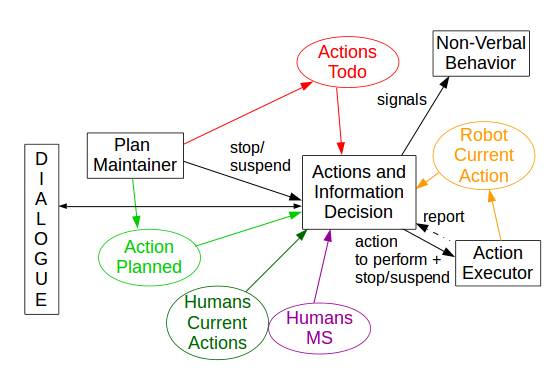
\includegraphics[width=0.7\textwidth]{figs/Chapter2/RobotDecision.png}
    \caption{Interaction of the Robot Decision module with the rest of the supervisor.}
    \label{fig:robotDecition}
\end{figure}

The Robot Decision module sends commands to the Action Executor from which it receives reports. It also communicates with the dialogue module and the Non-Verbal Behavior module to give the correct information.

\subsection{Action Executor}

The Action Executor is in charge of supervising robot actions. It receives actions to execute and stop or suspend orders from the robot decision and calls lower level modules to perform the given action in the best possible way. The action execution has been studied in this thesis and will be developed in Chapter \ref{ch:Acting}.

\begin{figure}[!h]
	\centering
    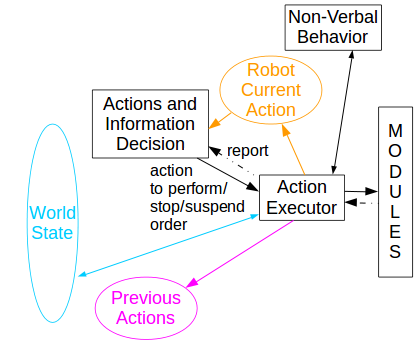
\includegraphics[width=0.5\textwidth]{figs/Chapter2/ActionExecutor.png}
    \caption{Interaction of the Action Executor with the rest of the supervisor.}
    \label{fig:actionExecutor}
\end{figure}

\newpage
\subsection{Non-Verbal Behavior}

This module allows to control the non-verbal behavior of the robot. In the current supervisor version, only the robot head behavior is concerned, but other type of non-verbal behaviors can be envisioned. The principles behind this module will be developed in Chapter \ref{ch:Acting}.

\begin{figure}[!h]
	\centering
    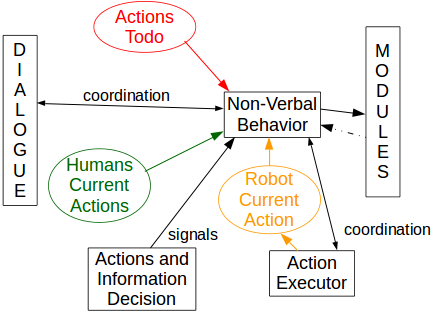
\includegraphics[width=0.5\textwidth]{figs/Chapter2/NVBehavior.png}
    \caption{Interaction of the Non-Verbal Behavior with the rest of the supervisor.}
    \label{fig:NVBehavior}
\end{figure}

The robot head behavior is based on the current robot action, the humans activities and the actions to perform. The module communicates with the dialogue module in order to coordinate and calls lower modules to control the robot. 

\section{Data representation}

\label{sec:data}

As seen in the previous section, several types of data are produced and used by the supervisor to take decisions. We will see now how we represent this data and this formalization will be used in the next chapters of the thesis.

The current state of the world from the robot point of view $WS$ is composed of a set of predicates $p$:
$$p = <entity, attribute, value>$$
For example, the fact that an object is on a table will be represented as $<object, isOn, table>$.

A goal $g$ is represented as:
$$g = <Name_g, Actors_g, Params_g, Obj_g>$$
where $Name_g$ allows to identify the goal, $Actors_g$ are the agents involved in the goal achievement, $Params_g$ are entities  (agents or objects) used to define precisely the goal and $Obj_g$ is a set of predicates representing the objective of the goal.
For example, if the robot has for goal to clean the table of the kitchen in collaboration with Bob by removing all items on it, this goal will be represented as:
$<Clean, <Robot, Bob>, <Kitchen\_table>, <<NULL, isOn, Kitchen\_table>>>$.
Finally, at its end, each goal $g$ is stored and associated with a label noted $label_g$ which can be equal either to DONE or ABORTED.

Then, a Shared Plan $SP$ is represented as:
$$SP = <id_p, A_p, L_p>$$
where $id_p$ is used to identify the plan, $A_p$ are the actions composing the plan and $L_p$ the links representing the order the actions should be executed (causal links).

A link $l \in L_p$ can be describe as:
 $$l = \langle prev_l, \ next_l \rangle$$
where $prev_l$ is the id of the action which needs to be achieved before the action with the id $next_l$ is performed. 

The actions composing the plan $A_p$ can be decomposed as:
$$A_p = <A_{prev}, A_{cur}, A_{next}, A_{later}>$$
where $A_{prev}$ are the actions of the plan already executed, $A_{cur}$ the actions currently executed, $A_{next}$ the actions which can be performed according to causal links and actions preconditions and $A_{later}$ the actions to be executed in the future.
Each of the set of actions previously introduced can be decomposed as:
$$<A = A^R, A^H, A^X>$$
where $A^R$ are the actions assigned to the robot, $A^H$ the actions assigned to the human and $A^X$ the actions not yet assigned. Indeed, we will see in Chapter~\ref{ch:SP} that not all actions are assigned to an actor during plan elaboration.
Finally, each action $a$ in $A_{prev}$ is associated with a label noted $label_a$ which can be equal either to DONE, FAILED or ABORTED.

An action $a$ can be represented as: 
$$a = < id_{a}, \ Name_{a}, \ Ag_{a}, \ Params_{a}, \ Precs_{a}, \ Effects_{a} >$$
Where $id_{a}$ is the action identifier and $Name_{a}$ represents its name. $Actors_{a}$ are the actors of the actions and $Params_{a}$ a set of parameters (objects or agents) which allows to define precisely the action. $Precs_{a}$ and $Effects_{a}$ are sets of predicates representing respectively the action preconditions and effects.
For example the action for the robot to place an object on a support will be defined as:$<0, place, Robot, <object, support>, <<object, isHoldBy, Robot>>, <<object, isOn, support>>>$.

The information concerning the state of the task is regrouped in what will be called the Task State $TS$:
$$TS = <g_R, SP, WS>$$
with $g_R$ the current goal of the robot, $SP$ the current Shared Plan and $WS$ the current world state from the robot point of view.

The robot also have a representation of humans mental state. The representation of the mental state $MS(H)$ of a human H is represented as:
$$MS(H) = <g_H, g_R(H), SP(H), WS(H)>$$
where $g_H$ is the goal the robot estimates the human is engaged in, $g_R(H)$ is the goal the robot estimates the human thinks the robot is performing, and $SP(H)$ and $WS(H)$ are the estimation of the Shared Plan and the World State from the human point of view.
$SP(H)$ is represented in the same way as the robot Shared Plan.


\ifdefined\included
\else
\bibliographystyle{StyleThese}
\bibliography{These}
\end{document}
\fi
